\section{System Architecture}
\label{sec:system}

\textsc{ScholAR} is a local interactive system: a Python/FastAPI backend prepares source-scoped evidence and a Next.js/React frontend presents the answer beside the document. Figure~\ref{fig:architecture} summarizes the three stages that matter to a reader: document representation, evidence retrieval and local answering, and verification and inspection.

\begin{figure*}[t]
\centering
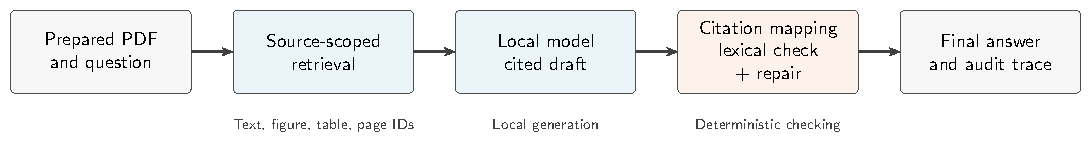
\includegraphics[width=\textwidth]{figs/architecture.pdf}
\caption{\textbf{Three-stage ScholAR pipeline.} A PDF becomes layout-aware evidence objects; hybrid retrieval supplies a local model with source-scoped context; verification and the interface keep the final answer connected to inspectable regions and an audit trace.}
\label{fig:architecture}
\end{figure*}

\subsection{Document representation}
When a user provides a scientific PDF, the ingestion engine extracts both structural semantics and visual coordinates:
\begin{itemize}[leftmargin=*,itemsep=1pt,topsep=2pt]
    \item A layout-aware parser recovers document hierarchy while isolating figures and tables, with a PyMuPDF fallback.
    \item Each text or visual element receives a source-scoped identity containing its document, page, and normalized bounding box.
    \item Figures, tables, and page regions remain available as local crops; ingestion commits atomically so a partial paper is not queryable.
\end{itemize}

\subsection{Evidence retrieval and local answering}
BM25 and dense text retrieval are fused with reciprocal-rank fusion; visual crops and full pages provide candidates when a question refers to a figure or table. The application---not the model---owns page numbers and bounding boxes. Retrieved evidence is placed in a structured prompt for a local Ollama model such as \texttt{qwen3.5:9b}; the model emits citation markers referring to evidence items, while the application maps those markers back to source identities. Strict-local mode blocks non-loopback network access during analysis, separating local answering from any explicitly enabled acquisition step.

\subsection{Verification and inspection}
After generation, \textsc{ScholAR} runs a post-generation inspection stage via \texttt{verifier\_service}:
\begin{itemize}[leftmargin=*,itemsep=1pt,topsep=2pt]
    \item lexical overlap and numerical checks flag mismatches between cited claims and supplied evidence;
    \item bounded remapping or pruning records changes without generating replacement facts; and
    \item the query, retrieved objects, raw completion, verifier actions, final citations, and timings are stored in a versioned trace that the Evidence Graph view exposes.
\end{itemize}
The verifier is a routing and inspection aid, not semantic entailment or human-verified ground truth. The user's central action remains direct inspection of the original PDF region.
